\chapter{Evaluation}\label{chap:test}
After producing the application described in Chapter~\ref{chap:imp}, referring
back to the design specifications to determine its performance against the
stated criteria was the next step.  

\section{Methodology}
Using a sample of e-mails provided by my supervisor, each of them was run
through the final version of the program, and scored based on the following
attributes:

\begin{itemize}
\item Let $M$ be the total number of received fields.
\item Let $N$ be the total number of other fields.
\item 1 point is added to the total $R$ for each piece of information found in a Received field for the following:
\begin{itemize}
\item{One of device name \emph{or} IP address}
\item{Software \emph{or} protocol used}
\item{Vulnerabilities found for the relevant piece of software}
\item{Location Data}
\end{itemize}
\item 1 point is addded to $F$ for each piece of information found in other fields.
\end{itemize}

The final score for an e-mail is given as \[\frac12\left(\frac R{4M}+\frac
FN\right)\]to give a value between 0 and 1 for each e-mail.

The e-mails received have been numbered from 1 up to 70, and a random sample of
size 30 was selected using the following code:

\begin{verbatim}
>>> random.seed()
>>> random.sample(list(range(1,70)), 30)
[64, 48, 11, 21, 63, 68, 27, 69, 29,  8, 28,
 34, 13, 57, 10,  3, 22, 32, 23, 49, 26, 45,
 19,  1, 36, 46, 41, 18, 20, 17]
\end{verbatim}

Thus giving a sorted list of the following e-mails: 1, 3, 8, 10, 11, 13, 17,
18, 19, 20, 21, 22, 23, 26, 27, 28, 29, 32, 34, 36, 41, 45, 46, 48, 49, 57, 63,
64, 68, 69.

\section{Sample Output}

The following pages show the results of running the completed software on the
e-mail labelled \texttt{11.txt}, the contents of which is listed in
Fragment~\ref{eg:11}.  The full table of CVE entries is elided for brevity.  
The entries in \colorbox{red!30}{this colour} are associated with points scored
for $R$, and the entries in \colorbox{blue!30}{this colour} are associated with
points scored for $F$.

\begin{example}[caption=Email \texttt{11.txt},label=eg:11]
Received: from relay13.mail.ox.ac.uk (129.67.1.163) by HUB01.ad.oak.ox.ac.uk 
 (|\colorbox{red!30}{163.1.154.218}|) with |\colorbox{red!30}{Microsoft SMTP Server}| id 14.3.169.1; Wed, 1 Apr 2015 
 11:06:18 +0100 
Received: from postie2.cs.ox.ac.uk ([129.67.151.44])	by |\colorbox{red!30}{relay12.mail.ox.ac.uk }|
 with |\colorbox{red!30}{esmtp (Exim 4.80}|)	(envelope-from <ahayes@mays.tamu.edu>)	id 
 1YdFXO-0008P8-de	for cccc1111@nexus.ox.ac.uk; Wed, 01 Apr 2015 11:06:18 +0100 
Received: from mailer.cs.ox.ac.uk ([129.67.151.81]:36787)	by 
 |\colorbox{red!30}{postie2.cs.ox.ac.uk}| with |\colorbox{red!30}{esmtp (Exim 4.72)}|	(envelope-from 
 <ahayes@mays.tamu.edu>)	id 1YdFWT-0004Fk-DZ	for jason.nurse@cs.ox.ac.uk; Wed, 
 01 Apr 2015 11:05:21 +0100 
Received: from relay11.mail.ox.ac.uk ([129.67.1.162]:57950)	by 
|\colorbox{red!30}{mailer.cs.ox.ac.uk}| with |\colorbox{red!30}{esmtp (Exim 4.72)}|	(envelope-from 
 <ahayes@mays.tamu.edu>)	id 1YdFWS-0003OY-6C	for jason.nurse@cs.ox.ac.uk; Wed, 
 01 Apr 2015 11:05:20 +0100 
Received: from mailbox2.mbs.tamu.edu ([128.194.216.125])	by 
|\colorbox{red!30}{relay11.mail.ox.ac.uk}| with |\colorbox{red!30}{esmtp (Exim 4.80)}|	(envelope-from 
 <ahayes@mays.tamu.edu>)	id 1YdFWS-0000Ck-Zf	for jason.nurse@cs.ox.ac.uk; Wed, 
 01 Apr 2015 11:05:20 +0100 
Received: from MAILBOX1.mbs.tamu.edu ([|\colorbox{red!30}{169.254.2.132}|]) by
MAILBOX2.mbs.tamu.edu ([|\colorbox{red!30}{169.254.1.80}|]) with |\colorbox{red!30}{mapi}| id 14.03.0224.002; Wed, 1
Apr 2015 05:05:00 -0500
From: |\colorbox{blue!30}{"Hayes, Allison" <ahayes@mays.tamu.edu>}|
To: "Hayes, Allison" <ahayes@mays.tamu.edu>
Subject: RE: ITS HELP DESK
Thread-Topic: ITS HELP DESK
Thread-Index: AdBsXNo2iPt2JIAvQzCkSflypfIvlgABOhlv
Date: Wed, 1 Apr 2015 10:04:57 +0000 
Message-ID: <3AC6BF6FEAFA734A8A0397E31CB7AD009B695F@MAILBOX1.mbs.tamu.edu> 
References: <3AC6BF6FEAFA734A8A0397E31CB7AD009A5A35@MAILBOX1.mbs.tamu.edu> 
In-Reply-To: <3AC6BF6FEAFA734A8A0397E31CB7AD009A5A35@MAILBOX1.mbs.tamu.edu> 
|\colorbox{blue!30}{Accept-Language: en-US }|
Content-Language: en-US 
X-MS-Has-Attach: 
X-MS-TNEF-Correlator: 
x-originating-ip: [208.76.111.246] 
Content-Type: multipart/alternative; 
	boundary="_000_3AC6BF6FEAFA734A8A0397E31CB7AD009B695FMAILBOX1mbstamued_" 
MIME-Version: 1.0 
X-Oxmail-Spam-Status: score=2.9 tests=HTML_MESSAGE,SUBJ_ALL_CAPS,T_RP_MATCHES_RCVD,URI_HEX 
X-Oxmail-Spam-Level: ** 
Return-Path: ahayes@mays.tamu.edu 
|\colorbox{blue!30}{X-MS-Exchange-Organization-AuthSource: HUB01.ad.oak.ox.ac.uk }|
|\colorbox{blue!30}{X-MS-Exchange-Organization-AuthAs: Anonymous }|
|\colorbox{blue!30}{X-MS-Exchange-Organization-AVStamp-Mailbox: Sophos;-2052447998;0;PM }|
|\colorbox{blue!30}{X-MS-Exchange-Organization-SCL: 2 }|
\end{example}

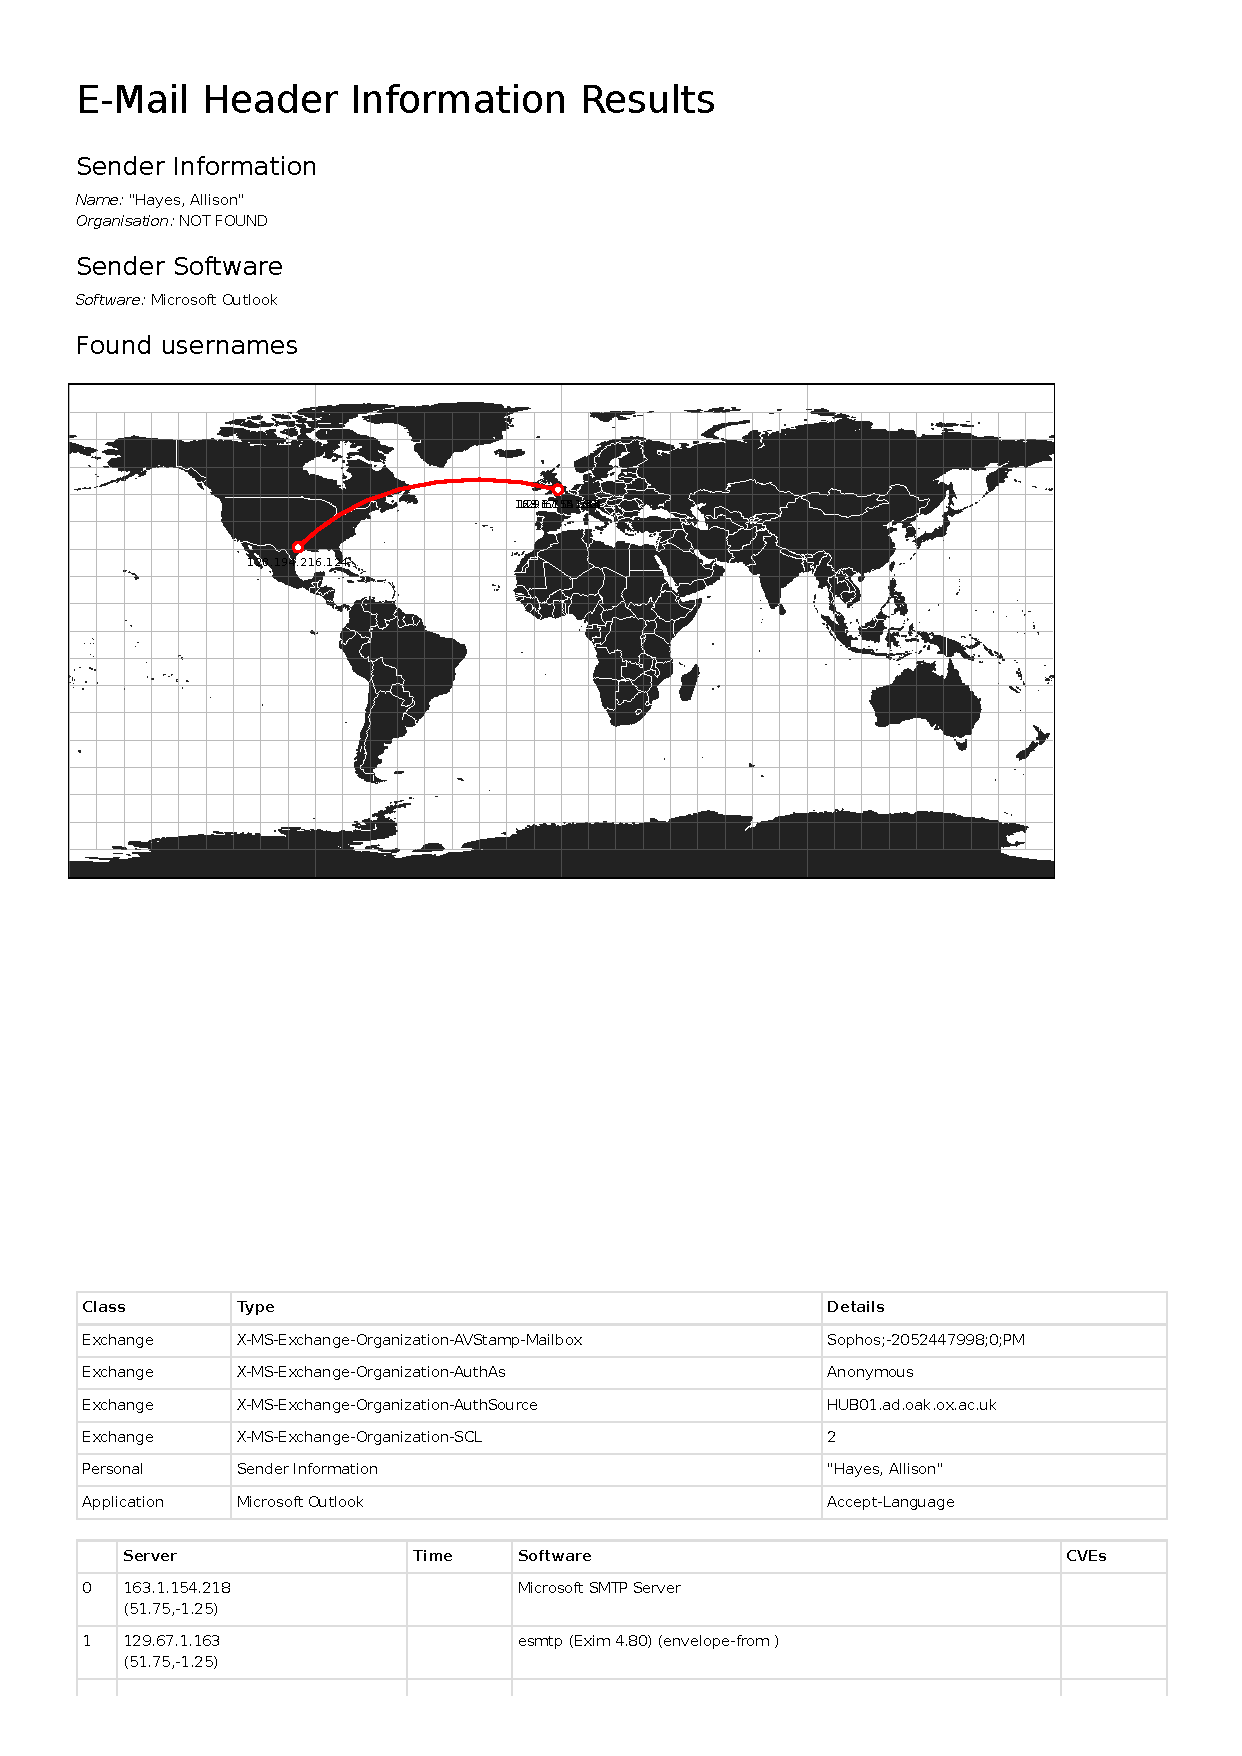
\includepdf[pages={1,2,3}]{11_results.pdf}

\section{Results}

Table~\ref{tab:sammn} gives the $M$ and $N$ values for the different sampled
e-mails.  These were sampled using standard Unix tools: \texttt{grep}ping for
fields and counting the output. The results for $R$ and $F$ have been listed
after completing the testing, after counting the number of entries in the final
visualisation.

\begin{table}
\centering
\begin{tabular}{@{}lrrrrrr@{}}
\toprule
Header & Total Fields &                  $M$  & $N$  & $R$ & $F$ & $S$ \\ \midrule
1.txt  & 26           & 7                     & 19   & 23  & 7   & 0.594924812    \\
3.txt  & 32           & 6                     & 26   & 16  & 6   & 0.4487179487   \\
8.txt  & 34           & 8                     & 26   & 30  & 6   & 0.5841346154   \\
10.txt & 22           & 3                     & 19   & 9   & 7   & 0.5592105263   \\
11.txt & 29           & 6                     & 23   & 23  & 6   & 0.6096014493   \\
13.txt & 17           & 4                     & 13   & 13  & 5   & 0.5985576923   \\
17.txt & 27           & 6                     & 21   & 22  & 6   & 0.6011904762   \\
18.txt & 20           & 6                     & 14   & 23  & 5   & 0.6577380952   \\
19.txt & 20           & 6                     & 14   & 21  & 4   & 0.5803571429   \\
20.txt & 22           & 7                     & 15   & 25  & 7   & 0.6797619048   \\
21.txt & 22           & 6                     & 16   & 23  & 5   & 0.6354166667   \\
22.txt & 22           & 6                     & 16   & 22  & 6   & 0.6458333333   \\
23.txt & 26           & 6                     & 20   & 20  & 7   & 0.5373563218   \\
26.txt & 19           & 6                     & 13   & 21  & 5   & 0.6298076923   \\
27.txt & 21           & 1                     & 20   & 2   & 8   & 0.45           \\
28.txt & 22           & 6                     & 16   & 23  & 4   & 0.6041666667   \\
29.txt & 20           & 6                     & 14   & 21  & 6   & 0.6517857143   \\
32.txt & 24           & 6                     & 18   & 20  & 3   & 0.5            \\
34.txt & 23           & 5                     & 18   & 19  & 4   & 0.586111111    \\
36.txt & 26           & 6                     & 20   & 21  & 4   & 0.5375         \\
41.txt & 21           & 6                     & 15   & 20  & 5   & 0.5833333333   \\
45.txt & 23           & 6                     & 17   & 22  & 5   & 0.6053921569   \\
46.txt & 26           & 5                     & 21   & 15  & 7   & 0.5416666667   \\
48.txt & 25           & 6                     & 19   & 22  & 6   & 0.6162280702   \\
49.txt & 21           & 6                     & 15   & 22  & 3   & 0.5583333333   \\
57.txt & 28           & 6                     & 22   & 21  & 4   & 0.5284090909   \\
63.txt & 23           & 5                     & 18   & 18  & 5   & 0.5888888889   \\
64.txt & 36           & 9                     & 27   & 31  & 6   & 0.5416666667   \\
68.txt & 21           & 6                     & 15   & 20  & 5   & 0.5833333333   \\
69.txt & 22           & 6                     & 16   & 21  & 5   & 0.59375        \\ \midrule
\emph{Average} & 24.3 & 5.8                   & 18.5 & 20.3& 5.4 & 0.582916135    \\ \bottomrule
\end{tabular}
\caption{$M$, $N$, $R$, $F$ and score values for chosen headers}
\label{tab:sammn}
\end{table}

\begin{figure}
	\centering\resizebox{0.75\textwidth}{!}{
\begin{tikzpicture}
\begin{axis}[
    ybar,
    ymin=0
]
\addplot +[
    hist={
        bins=10,
        data min=0.4,
        data max=0.7
    }   
] table [y index=0] {data.csv};
\end{axis}
\end{tikzpicture}}
\caption{Distribution of scores from e-mails}\label{fig:dis}
\end{figure}

The final score for the e-mails gives a minimum value of 0.449 and a maximum
value of 0.680, with an average of 0.583 and standard deviation of 0.0540. The
histogram in Figure~\ref{fig:dis} shows the distribution of scores from the
e-mails, showing a skew towards higher scores.  This is a promising result,
however, most of the score is contributed to by the trace-fields, with the 
value of $R/4N$ being consistently around 0.85.  As the aim of this project
jas both focused on the disclosure of individual's data and of network
vulnerabilities, the high score from the trace-fields is a positive result.

During the testing, the following trends were noticed.  As many of the e-mails
passed through the same set of servers, as they had been received by an Oxford
e-mail address, the same set of servers were frequently seen, all of which had
associated IP addresses, geolocation data and (except for one server running
Microsoft SMTP Server) CVE data for the running software.  For an e-mail sent
within the University Nexus system, this gives an inflated score, as very few
of the servers are missing information.

The score for the information gathered from fields does not take into account
the number of fields needed to determine or infer a piece of information. For
example, the presence, or absence of multiple fields is required to determine a
piece of information.  Nor does it consider the relative value of a piece of
information, failing to rate the presence of a username above the presence of a
particular piece of software also giving false positives.

However, very few e-mails in the testing population contained fields relating
to usernames (for example, \texttt{X-}$\ldots$\texttt{-User}, \texttt{X-Oxford-Username},
\texttt{X-Authenticated-User}) compared to the result
in~\cite{nurse2015investigating}, which found 14\% of e-mails to contain
usernames as opposed to the 8\% found in the population.

\cleardoublepage \chapter{Evaluation}
\section{Conclusions}

As described in Chapter~\ref{chap:int}, the aim of this project is to support a
better understanding of the data that may leaked when e-mails are sent, both
from a personal perspective, as well as the corporate data that is leaked
concern network configurations and software installations.

To support this, I have developed a tool that can be used to automatically
extract information from e-mail headers and analyse its results to display the
personal information contained within an e-mail's header, as well as
information about the software configurations that may be found on a user's
computer, or the servers used to send their e-mail.


\section{Future Work}

During the late stages of development and testing, a number of missing features
quickly became apparent. Due to the limited information available, and the
differences in version numbering, a decision was made to search for all
available vulnerabilities for an application, allowing the user to discern
which were most relevant.  Subsequent versions could focus on the different
pieces of version data available.  For example, \texttt{esmtp} frequently
references its version number in the ``Received'' field frequently.

Alternatively, a better picture may be presented by accumulating multiple
e-mails. For example, using the information provided from multiple members of
single organisation, a better picture may be built up of the software used by
the servers, as well as the network configuration.

The application's response times may also be improved by caching some data in
memory, such as WhoIs responses and GeoIP lookups, so that frequently accessed
lookups can be completed more quickly.

Additionally, future testing should take place on a larger dataset, using
e-mails from a wider variety of sources sent to a number of different
recipients.  

Finally, it should be possible for an updated version of this application to
determine which header fields have been added by mail servers within one's own
organisation.  For example, e-mail header fields beginning with
\texttt{X-MS-Exchange} are seen within almost all e-mail messages sent to
recipients within the Oxford domain, adding more false positives to the test
results. While it is possible that other preceding e-mail servers have added
similar fields, in most cases, these entries yielded little useful data.

